\relax
\section{電磁固有モード}
\paragraph{縦波モードとプラズモン}
半導体や誘電体では,価電子帯から伝導体に励起した電子と,価電子帯に残った正孔がクーロン力で結合して励起子(エキシトン)ができる.
励起子はクーロン力で結合しているので,エネルギー的に若干安定していることになる.金属でも励起子はできるが,その存在時間はとても短く観測は困難である.
最近(2017年現在)銀の励起子の寿命が長いことが分かったらしい.そのような励起子と電磁場の相互作用を考える.
まずは等方的な物質中のMaxwell方程式を記述しよう:
\begin{align}
  \dive \boldsymbol{D} &= \rho\label{long_mode_gauss}, \\
  \rot \boldsymbol{E} &= -\dfrac{\partial\boldsymbol{B}}{\partial{t}}, \\
  \rot \boldsymbol{H} &= \boldsymbol{j} + \dfrac{\partial\boldsymbol{D}}{\partial{t}}, \\
  \dive \boldsymbol{B} &= 0.
\end{align}
内部に存在する電場は
\begin{align}
  \boldsymbol{E} = \boldsymbol{E}_0\exp\left[i(\boldsymbol{k}\cdot\boldsymbol{r}-\omega{t})\right]
\end{align}
とする.これを(\ref{long_mode_gauss})に代入すると,
\begin{align}
  i\varepsilon(\omega)\boldsymbol{k}\cdot\boldsymbol{E}=\rho
\end{align}
となる.ただし,$\varepsilon(\omega)$は誘電関数である.
よって,これを解くと,
\begin{align}
  \boldsymbol{E}=\boldsymbol{E}_l=-\dfrac{i\boldsymbol{k}}{k^2\varepsilon(\omega)}\rho\label{long_mode_El}
\end{align}
となる.これは電場の波(電磁波でないことに注意)の進む方向$\boldsymbol{k}$に平行なので,縦波である.
外部電荷密度$\rho=0$の時には$E_l=0$となるが,振動子モデルで調べたように,散逸を無視した拡張振動子の誘電関数は,
\begin{align}
  \varepsilon(\omega)=\varepsilon_\text{b}+\dfrac{\varepsilon_0}{{\omega_0}^2-\omega^2}\dfrac{nq^2}{\varepsilon_0m}\label{long_mode_permittivity}
\end{align}
で与えられる.この場合は,常に$\varepsilon(\omega)=0$となる$\omega=0$が存在するので,(\ref{long_mode_El})において,$\rho=0$であっても$\boldsymbol{E}_l\neq0$となり,縦波が存在する.
以上から,縦波が存在する条件は,
\begin{align}
  \varepsilon(\omega)=0\label{long_mode_lwave}
\end{align}
である.また,この条件を満たす角振動数$\omega$は,(\ref{long_mode_permittivity})と(\ref{long_mode_lwave})から,
\begin{align}
  \omega=\omega_l=\sqrt{{\omega_0}^2+\dfrac{\varepsilon_0}{\varepsilon_\text{b}}\dfrac{nq^2}{\varepsilon_0m}}
\end{align}
となる.これを縦波の角振動数と言う.さらに,金属や電離気体では,原子核と電子間の束縛がなく,弾性定数$K=0$なので$\omega_0=0$となる.
このような物質をプラズマと言う.プラズマにおいて$\varepsilon_\text{b}=\varepsilon_0$の時の縦波の角振動数
\begin{align}
  \omega_l=\omega_p=\sqrt{\dfrac{nq^2}{\varepsilon_0m}}
\end{align}
をプラズマ角振動数と言う.

上で求めた条件(\ref{long_mode_lwave})を別の方法で導いてみよう.
物質の中に波数$\boldsymbol{k}$で表される電気分極$\boldsymbol{P}$の縦波平面波があるとする.
この時,分極電荷による反電場$\boldsymbol{E}$を考えることができるので(本当はある一点の周りの電気双極子モーメントによる電場が存在している),
\begin{align}
  \boldsymbol{E}=-\dfrac{\boldsymbol{P}}{\varepsilon_0}
\end{align}
である.さらに,$\boldsymbol{P}=\varepsilon_0\chi\boldsymbol{E}$を代入すると,$\chi=-1$となる.
これを誘電率と電気感受率の関係式$\varepsilon=\varepsilon_0(1+\chi)$に代入すると,確かに
\begin{align}
  \varepsilon=0
\end{align}
となる.プラズマの場合,縦波を発生させる復元力を担っているものは反電場なのである.
また,波の位相とほぼ等速で進む電子が電磁波の電場によってエネルギーを得るため,縦波は減衰する.これをLandau減衰と呼ぶ.
プラズマ中の自由電子は集団的に振動しているので,擬似的な粒子(量子)として振舞っていると考えることができる.これをプラズモンという.
角振動数$\omega_p$で振動するプラズモンは$\hbar\omega_p$のエネルギーを持つことのみが許される.

\paragraph{横波モードとポラリトン}
励起子と電磁場の相互作用系の縦波では,伝播する変化である電気分極$\boldsymbol{P}$に対する復元力は反電場$\boldsymbol{E}$であった.

電荷がない時のMaxwell方程式は,
\begin{align}
  \varepsilon(\omega)\boldsymbol{k}\cdot\boldsymbol{E}=0
\end{align}
となる.$\varepsilon(\omega)\neq0$の領域では,$\boldsymbol{k}\perp\boldsymbol{E}$となり,これは横波である.

拡張された電磁波動方程式\eqref{comp_wave_eq_newequationE}において散逸$\gamma$を無視したとき,波数$k$と角振動数$\omega$の分散は,
\begin{align}
  k^2=\mu_0\varepsilon_0\left(\dfrac{\varepsilon_{\text{b}}}{\varepsilon_0}+\dfrac{{\omega_p}^2}{{\omega_0}^2-\omega^2}\right)\omega^2\label{trans_mode_div}
\end{align}
で与えられる.
左辺が正なので,右辺も正でなくてはならない.よって,$\omega$が存在できる範囲は,
\begin{align}
  \omega < \omega_0 , \quad  \omega > \sqrt{{\omega_0}^2+\dfrac{\varepsilon_0}{\varepsilon_{\text{b}}}{\omega_p}^2} = \omega_l
\end{align}
となる.$\omega_l$は縦波の各振動数,$\omega_p$はプラズマ角振動数である.
(\ref{trans_mode_div})を図示すると,本文図8-19のようになる.
分散曲線が2本に分かれるのは,誘電率$\varepsilon_{\text{b}}$の物質中を進む電磁波$(\omega=c_{\text{b}}k)$と誘電体内の分極の振動$(\omega=\omega_0)$の混合状態だからである.
これをポラリトンという.

$\omega\ll\omega_0$の時は\eqref{osc_model_st}の静的な誘電率$\varepsilon_{\text{st}}$に従って速さ$c_{\text{s}}=\dfrac{c}{\sqrt{\varepsilon_{\text{st}}}}$で進む電磁波となる.

$\omega\to\omega_0-0$の時は$k,\varepsilon\to\infty$となり,これは背景媒質に関係ない分極の波になる.
なぜならば,背景媒質とは注目している分極の固有角振動数$\omega_0$よりも大きな固有角振動数を持つもののことを言うからである.
ここでは注目している分極が共鳴を起こし,背景媒質の寄与はとても小さくなる.

$\omega\to\omega_l+0$の時は$k,\varepsilon\to0$となり,これは縦波と同じ状況である.

$\omega\gg\omega_0$となると,固有角振動数$\omega_0$の分極の寄与はほとんどなくなる.その結果一定の背景媒質を進む電磁波となる.

\paragraph{プラズマの表皮効果}
プラズマに入射する電磁波のふるまいを見よう.プラズマで散逸$\gamma$が小さいとすると, 振動子モデルで考えた拡張した誘電関数において$\varepsilon_{\text{b}}=\varepsilon_0$として,
\begin{align}
  \varepsilon(\omega)=\varepsilon_0\left(\dfrac{\omega^2-{\omega_p}^2}{\omega^2}\right)
\end{align}
となる.よって,$\omega < \omega_p$のときは誘電関数が負となる.波動方程式\eqref{comp_wave_eq_newequationE}から,
\begin{align}
  n&=0\label{skin_eff_n}\\
  \kappa&=\dfrac{\sqrt{{{\omega_p}^2-\omega^2}}}{\omega}\label{skin_eff_kappa}
\end{align}
となる.$\omega_p$の値は,通常の金属では$10^{16}$程度である.これに対して可視光の$\omega$は$10^{15}\sim10^{16}$程度である.
よって,金属でほとんどの光が反射される.だが,それでも一部の光は減衰しながら金属中に侵入する.
$x$軸に伝わる電磁波を考える.$0\leq{x}$の適当な範囲にプラズマが存在するとしよう(本文図8-9みたいな感じ).

(\ref{skin_eff_n})と(\ref{skin_eff_kappa})を減衰を考えた電場\eqref{comp_wave_eq_E}に代入して,
\begin{align}
  \boldsymbol{E}=\boldsymbol{E}_0\exp\left(-\dfrac{\sqrt{{{\omega_p}^2-\omega^2}}}{c}x\right)\exp(-i\omega{t})
\end{align}
を得る.これは,$x$軸方向に減衰する波を表す.この式からも分かるように,波は薄いプラズマ中では完全に0になる訳ではない.このようなものを消衰波と言う.
静電場がかかっていればプラズマ中では静電誘導により電場が0となるが,これは時間的に変動する電場なので静電誘導は起こらない.電磁波の場合は消衰波ができ,電場が弱くなる.
これを表被効果という.

\paragraph{ヘリコン波とホイスラー波}
プラズマ角振動数$\omega_p$より角振動数$\omega$が小さい電磁波はプラズマ中では伝播できないことが分かった.
だが,特別な場合はそのような電磁波であっても伝播できる.

\eqref{e_diople_in_m_tensor}から,$\zeta$方向に磁場がかかっている時の感受率テンソルは,
\begin{align}
  \chi =
  \dfrac{{\omega_p}^2}{\omega}\left(
  \begin{array}{ccc}
    \dfrac{\omega+i\gamma}{{\omega_c}^2-(\omega+i\gamma)^2} & \dfrac{i\omega_c}{{\omega_c}^2-(\omega+i\gamma)^2} & 0 \\ \\
    \dfrac{-i\omega_c}{{\omega_c}^2-(\omega+i\gamma)^2} & \dfrac{\omega+i\gamma}{{\omega_c}^2-(\omega+i\gamma)^2} & 0 \\ \\
    0 & 0 & \dfrac{-1}{\omega+i\gamma}
  \end{array}
  \right)
\end{align}
である.プラズマなので$\omega_0=0$である.散逸$\gamma$を無視すれば,
\begin{align}
  \chi =
  \dfrac{{\omega_p}^2}{\omega}\left(
  \begin{array}{ccc}
    \dfrac{\omega}{{\omega_c}^2-\omega^2} & \dfrac{i\omega_c}{{\omega_c}^2-\omega^2} & 0 \\ \\
    \dfrac{-i\omega_c}{{\omega_c}^2-\omega^2} & \dfrac{\omega}{{\omega_c}^2-\omega^2} & 0 \\ \\
    0 & 0 & -\dfrac{1}{\omega}
  \end{array}
  \right)
  \label{helicon_tensor}
\end{align}
$\zeta$正の向きに進む円偏光の電場は,
\begin{align}
  E_{\xi} &= iE_{\eta} , \quad  E_{\zeta}=0 ~ (\text{Right}) \label{helicon_right}\\
  E_{\eta} &= iE_{\xi} , \quad E_{\zeta}=0 ~ (\text{Left}) \label{helicon_left}
\end{align}
である.背景媒質$\varepsilon_{\text{b}}$でのポラリトンに対する拡張誘電関数は
\begin{align}
  \boldsymbol{D} &= \varepsilon_{\text{b}}\boldsymbol{E}+\boldsymbol{P}\notag\\
  &= \varepsilon_{\text{b}}\boldsymbol{E}+\varepsilon_0\chi\boldsymbol{E}\notag\\
  &= \varepsilon\boldsymbol{E}
\end{align}
このように決定される.ここで,一般に$\chi$と$\varepsilon$は2階のテンソルであるが,これを0階のテンソルに直すことを考える.右周りの円偏光に対しては,
\begin{align}\left(
  \begin{array}{c}
    D_{\xi} \\
    D_{\eta} \\
    D_{\zeta}
  \end{array}
  \right)
  &=
  \varepsilon_{\text{b}}
  \left(
  \begin{array}{c}
    iE_{\eta} \\
    E_{\eta} \\
    0
  \end{array}
  \right)
  +
  \dfrac{\varepsilon_0{\omega_p}^2}{\omega}\left(
  \begin{array}{ccc}
    \dfrac{\omega}{{\omega_c}^2-\omega^2} & \dfrac{i\omega_c}{{\omega_c}^2-\omega^2} & 0 \\ \\
    \dfrac{-i\omega_c}{{\omega_c}^2-\omega^2} & \dfrac{\omega}{{\omega_c}^2-\omega^2} & 0 \\ \\
    0 & 0 & -\dfrac{1}{\omega}
  \end{array}
  \right)
  \left(
  \begin{array}{c}
    iE_{\eta} \\
    E_{\eta} \\
    0
  \end{array}
  \right)\notag\\
  &=
  \left[\varepsilon_{\text{b}}+\dfrac{\varepsilon_0{\omega_p}^2}{\omega(\omega_c-\omega)}\right]
  \left(
  \begin{array}{c}
    iE_{\eta} \\
    E_{\eta} \\
    0
  \end{array}
  \right)
\end{align}
よって,右回りの円偏光に対する誘電率は
\begin{align}
  \varepsilon_{\text{R}}=\varepsilon_{\text{b}}+\dfrac{\varepsilon_0{\omega_p}^2}{\omega(\omega_c-\omega)}\label{helicon_perR}
\end{align}
で与えられる.同様に,左回りの円偏光に対する誘電率は
\begin{align}
  \varepsilon_{\text{L}}=\varepsilon_{\text{b}}-\dfrac{\varepsilon_0{\omega_p}^2}{\omega(\omega_c+\omega)}\label{helicon_perL}
\end{align}
で与えられる.$\omega_c=\dfrac{qB}{m}$はプラズマの荷電粒子と同じ符号を持つ.
よって,荷電粒子が正孔などの場合は$\varepsilon_{\text{R}}$,自由電子などの場合は$\varepsilon_{\text{L}}$が極を持つ.
$|\omega_c|$と$\omega$が一致するということは,サイクロトロン運動する荷電粒子と電磁波が共鳴するということである.これをサイクロトロン共鳴と言う.
ところで,(\ref{helicon_perR})と(\ref{helicon_perL})において$\omega$が十分小さいときは,
\begin{align}
  \varepsilon_{\text{R}} &= \dfrac{\varepsilon_0{\omega_p}^2}{\omega\omega_c}\label{helicon_perHR}\\
  \varepsilon_{\text{L}} &= -\dfrac{\varepsilon_0{\omega_p}^2}{\omega\omega_c}\label{helicon_perHL}
\end{align}
と近似される.荷電粒子が正孔などの場合は$\varepsilon_{\text{R}} > 0$となり右回りの偏光のみが伝播する.
一方で自由電子などの場合は$\varepsilon_{\text{L}} > 0$となり左回りの偏光のみが伝播する.

表皮効果で調べたように,プラズマ角振動数$\omega_p$より角振動数$\omega$が小さい電磁波はプラズマの中では減衰してしまう.
だが,磁場が存在するとプラズマ振動数よりも低い振動数の電磁波も伝わることができる.この波は電磁波とサイクロトロン運動の混成波で,ヘリコン波と言う.
ヘリコン波の分散は,ヘリコン波の角振動数を$\omega_\text{H}$とすると,
\begin{align}
  \varepsilon\mu_0=\dfrac{k^2}{{\omega_\text{H}}^2}
\end{align}
に(\ref{helicon_perHR}),(\ref{helicon_perHL})を代入して,
\begin{align}
  \omega_{\text{H}}=\dfrac{|\omega_c|}{\varepsilon_0\mu_0{\omega_p}^2}k^2=\dfrac{H}{n|q|}k^2
\end{align}
で与えられる.ただし,$H$は磁場の大きさである.

これと同じことが地球表面で起きており,電離層中を地磁気に沿って伝搬する電磁波をホイスラー波と呼ぶ.
南半球で発生した雷の信号が地磁気の磁力線に沿ってホイッスル状の雑音として北半球まで伝わることからこの名前がついている.

\paragraph{表面ポラリトン}
散逸を$\gamma$を無視した横波において,その分散は,
\begin{align}
  k^2=\mu_0\varepsilon_0\left(\dfrac{\varepsilon_{\text{b}}}{\varepsilon_0}+\dfrac{{\omega_p}^2}{{\omega_0}^2-\omega^2}\right)\omega^2
  \label{surface_traDiv}
\end{align}
で表される.これが横波として減衰せずに存在するためには,両辺正であることが必要である.
複素電磁方程式で導入した複素波数ベクトル\eqref{comp_wave_eq_Ek}において,虚部が正であれば減衰が起こるのであった.
よって,(\ref{surface_traDiv})において比誘電率$\tilde{\varepsilon}$が,
\begin{align}
  \tilde{\varepsilon}=\dfrac{\varepsilon_{\text{b}}}{\varepsilon_0}+\dfrac{{\omega_p}^2}{{\omega_0}^2-\omega^2} < 0
\end{align}
であれば横波はすぐに消衰し,表面のみに存在できることが分かる.

\begin{figure}[ht]
  \centering
  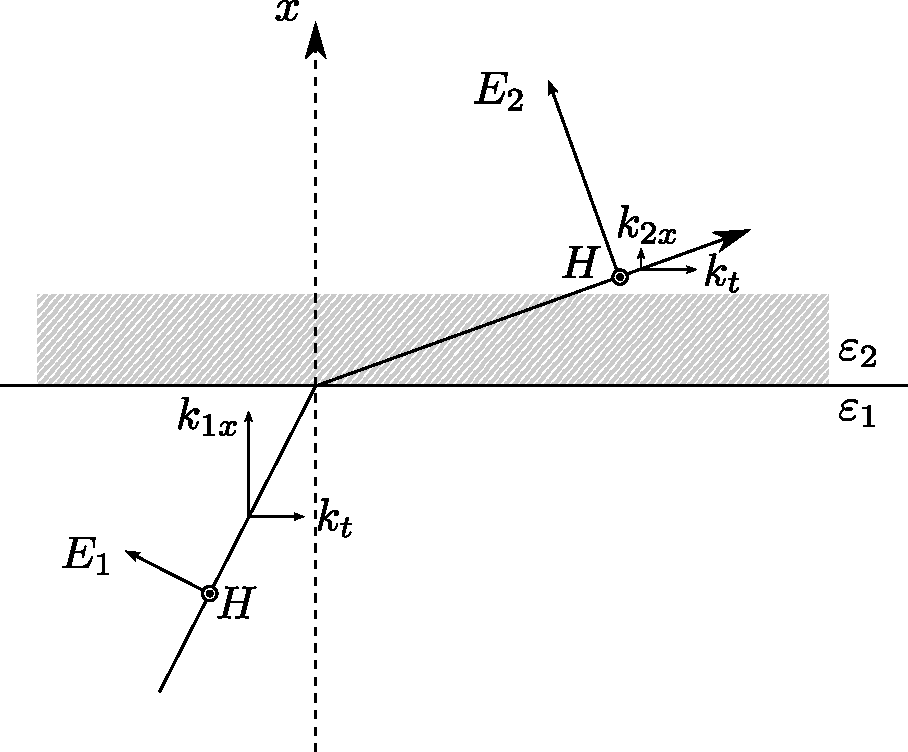
\includegraphics[scale=0.5]{TMrec.pdf}
  \caption{電磁波はTM波(磁場が入射面に平行な波;p偏光)とする}
  \label{TMrec}
\end{figure}

ここで,図のように誘電率$\varepsilon_1$の物質から誘電率$\varepsilon_2$の物質に入射する電磁波を考える.
電磁波の屈折や透過,反射において反射面に平行な波数は変化しないので,それを$k_t$とおいた.
両方の物質内で,電荷が存在しないとすると$\dive\boldsymbol{D}=0$なので,
\begin{align}
  k_tE_{1t}+k_{1x}E_{1x}=0\label{surface_E1} \\
  k_tE_{2t}+k_{2x}E_{2x}=0\label{surface_E2}
\end{align}
となる.さらに,境界において,電場の面に接する向きの成分は連続であり,電束密度の法線方向は連続であるので,
\begin{align}
  E_{1t}&=E_{2t}=E_t\label{surface_E} \\
  \varepsilon_1E_{1x}&=\varepsilon_2E_{2x}\label{surface_D}
\end{align}
となる.(\ref{surface_E1}),(\ref{surface_E2}),(\ref{surface_E}),(\ref{surface_D})から,
\begin{align}
  \varepsilon_2k_{1x}=\varepsilon_1k_{2x}\label{surface_epsK}
\end{align}
となる.両物質で透磁率がともに$\mu_0$であるとすると,電磁波の屈折や透過,反射において$\omega$は変化しないことから,
\begin{align*}
  \dfrac{\omega^2}{{k_{1t}}^2+{k_{1x}}^2}=\dfrac{\omega^2}{{k_1}^2}={c_1}^2=\dfrac{1}{\mu_0\varepsilon_1}=\dfrac{1}{\mu_0\varepsilon_0}\dfrac{\varepsilon_0}{\varepsilon_1}
  =c^2\dfrac{\varepsilon_0}{\varepsilon_1}=\dfrac{\omega^2}{{k}^2}\dfrac{\varepsilon_0}{\varepsilon_1}
\end{align*}
などの計算をして,
\begin{align}
  {k_{1t}}^2+{k_{1x}}^2=\dfrac{\varepsilon_1}{\varepsilon_0}k^2\label{surface_k1} \\
  {k_{2t}}^2+{k_{2x}}^2=\dfrac{\varepsilon_2}{\varepsilon_0}k^2\label{surface_k2}
\end{align}
となる.ただし,$k$は真空中での波数である.(\ref{surface_epsK}),(\ref{surface_k1}),(\ref{surface_k2})から,
\begin{align}
  {k_{1x}}^2&=\dfrac{{\varepsilon_1}^2}{\varepsilon_0(\varepsilon_1+\varepsilon_2)}k^2\label{surface_k1x}\\
  {k_{2x}}^2&=\dfrac{{\varepsilon_2}^2}{\varepsilon_0(\varepsilon_1+\varepsilon_2)}k^2\label{surface_k2x}\\
  {k_{t}}^2&=\dfrac{\varepsilon_1\varepsilon_2}{\varepsilon_0(\varepsilon_1+\varepsilon_2)}k^2\label{surface_kt}\\
\end{align}
となる.ここで,$k_t$が実数の下で$\varepsilon_1$の物質と$\varepsilon_2$の物質の中で電磁波が共に消衰波となるのは,
\begin{align}
  {k_{1x}}^2 < 0 \quad \text{かつ} \quad {k_{2x}}^2 < 0
\end{align}
の時である.(\ref{surface_k1x}),(\ref{surface_k2x})から,これは
\begin{align}
  \varepsilon_1\varepsilon_2 < 0 \quad \text{かつ} \quad \varepsilon_1+\varepsilon_2 < 0\label{surface_epsCond}
\end{align}
に対応する.この時,波は両側で消衰波となり,表面にのみ局在できる.

$\varepsilon_2$を拡張振動子モデルで散逸を無視したものとすると,
$\varepsilon_1$が真空で,$\varepsilon_2$の散逸$\gamma$が十分小さいときは,(\ref{surface_kt})から,
\begin{align}
  k_t=\dfrac{\omega}{c}\sqrt{\left(\dfrac{\varepsilon_{\text{b}}}{\varepsilon_0}+\dfrac{{\omega_p}^2}{{\omega_0}^2-\omega^2}\right)
  \left(1+\dfrac{\varepsilon_{\text{b}}}{\varepsilon_0}+\dfrac{{\omega_p}^2}{{\omega_0}^2-\omega^2}\right)^{-1}}
\end{align}
となる.ただし,(\ref{surface_epsCond})から,
\begin{align}
  \tilde{\varepsilon}_2=\dfrac{\varepsilon_{\text{b}}}{\varepsilon_0}+\dfrac{{\omega_p}^2}{{\omega_0}^2-\omega^2} < -1
\end{align}
である.これを変形すると,$\omega$の存在範囲は,
\begin{align}
  \omega_0+0 < \omega < \sqrt{{\omega_0}^2+\dfrac{\varepsilon_0}{\varepsilon_0+\varepsilon_{\text {b}}}{\omega_p}^2}=\omega_s
\end{align}
となる.この$\omega_s$を表面プラズマ角振動数と呼ぶ.
以上から,表面波の分散は,本文図8-21のようになる.

このような表面波を表面波ポラリトンと呼ぶ.これは,分極電荷の振動と電磁波の混成である.
表面波ポラリトンは,波数$k_t$で表面に沿って伝播する.
誘電体表面には,面密度$\sigma_P=P_n(\boldsymbol{r})$の分極電荷が分布していると考えることができるのであった.
よって,分極電荷の振幅は,
\begin{align}
  \sigma_P&=-P_{2x}\notag\\
  &=-D_{2x}-\varepsilon_0E_{2x}\notag\\
  &=-(\varepsilon_2-\varepsilon_0)E_{2x}\notag\\
  &=-i(\varepsilon_2-\varepsilon_0)\dfrac{k_t}{|k_{2x}|}E_t
\end{align}
となる.$x$軸の向きは誘電体の内側に向かっている.
$\varepsilon_2 < 0$より,$E_t$の位相は$\sigma_P$の位相より$\dfrac{\pi}{2}$遅れていることが分かる.
